\documentclass[11pt, a4paper]{article}

\usepackage{color}

\usepackage{amsmath}
\usepackage{amssymb}
\usepackage[pdftex]{graphicx}
\usepackage{alltt}
\usepackage{caption}
\usepackage{subcaption}
\usepackage{epstopdf}


\author{Yacine Derouach, Stefan Hegglin, Huub Heijnen, Elise Ledieu}
\title{Epidemic models of Flu outbreaks}
\begin{document}
\maketitle

\section{Model description}
\subsection{The SIR model}
\paragraph{}
The Susceptible-Infected-Recovered (SIR) model is a deterministic model that can be used to describe the influenza transmission. We consider the version proposed by Coehlo et al. [2].

\begin{equation}
\frac{dS}{dt} = - \lambda S
\end{equation}
\begin{equation}
\frac{dI}{dt} = \lambda S - \tau R
\end{equation}
\begin{equation}
\frac{dR}{dt} = \tau R
\end{equation}

with \[ \lambda = \beta (\alpha I + m) \]

where $S$ is the normalized number of susceptible individuals, $I$is the normalized number of infected individuals, $R$ is the normalized number of recovered individuals, $\tau $ is the recovery rate, $\beta $ is the transmission rate, $\alpha$ is the ratio of symptomatic infection and m is the infectious migration rate.

\begin{figure}[h]
\center
   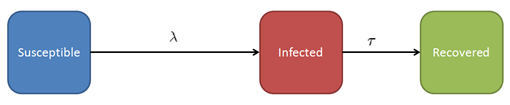
\includegraphics[width = \textwidth]{picture1.png}
   \caption{\label{1} Compartmental representation of the SIR model}
\end{figure}

$\beta$ is time-dependent and models the seasonality of the flu epidemics. Here, a sufficiently large step function is chosen (Figure ...).

%% ADD A FIGURE OF THE STEP FUNCTION USED

The set of parameters to be determined in this case is : $ { \alpha, \tau, m, S_o}$. $S_o$ is the number of susceptible individuals at the beginning at each season. The parameters $m$ and $\tau$ do not depend on the season considered, whereas the parameters $\alpha$ and $S_o$ change at each season.

\subsection{The SEIR model}
\paragraph{}
The Susceptible-Exposed-Infected-Recovered (SEIR) model is an extension of the SIR model. We added the Exposed category to the previous system.

\begin{equation}
\frac{dS}{dt} = - \lambda S
\end{equation}
\begin{equation}
\frac{dE}{dt} = \lambda S - \gamma E
\end{equation}
\begin{equation}
\frac{dI}{dt} = \gamma E - \tau R
\end{equation}
\begin{equation}
\frac{dR}{dt} = \tau R
\end{equation}

with \[ \lambda = \beta (\alpha I + m) \]

where $E$ is the normalized number of exposed individuals and $\gamma$ is the transition rate from latent to infected state.

\begin{figure}[h]
\center
   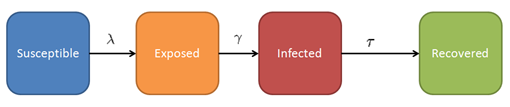
\includegraphics[width = \textwidth]{picture2.png}
   \caption{\label{2} Compartmental representation of the SEIR model}
\end{figure}


The set of parameters to be determined in this model is : $ { \alpha, \gamma, \tau, m, S_o}$. Here, we suppose that $\gamma$ is constant for all the seasons.

\section{Likelihood}
\paragraph{}
The likelihood of the parameters is 
\begin{equation}
L(\Theta) = L(\Phi) = \prod_{t=1}^T p( d(t) | \Phi(t),I) = \prod_{k=1}^K \prod_{t=1}^T p( d(t) | \Phi_k(t),I) 
\end{equation}

assuming normal errors with fixed variance $\sigma^2$
\begin{equation}
p(d(t) | \Phi_k(t),I) = \frac{1}{\sqrt{2\pi}\sigma} \exp^{-\frac{1}{2\sigma^2}[y(t) - I(x(t), \Theta)]}
\end{equation}

where $I(x(t), \Theta)$ is the number of infected people at time $t$ predicted by the model given the input values $x(t)$ ; $y(t)$ is the observed data ; $d(t)$ is the data at a time point.

$I(x(t), \Theta)$ corresponds to the solution of an ODE system. There may be no simple analytical solution for this one and therefore, no analytical derivation possible of it. It depends indeed on the parameter $\beta$, which is time-dependent.

\section{Priors}
\paragraph{}
Thanks to the article by Coehlo et al. [2], it is possible to use informative priors for the SIR model. By analogy, the information on the parameters in the SIR model is reused to determine the priors of the SEIR model. The $\gamma$ parameter has an uninformative prior (a uniform distribution between 0 and 1). Moreover, the prior over $\tau$ is considered to be uniform between 1 and 2, as it was derived experimentally in the article of Coehlo et al.. 

Here are the priors used for each parameter : 
\begin{itemize}
\item $\alpha \sim \mathcal{U}(0, 0.4)$ 
\item $\gamma \sim \mathcal{U}(0, 1)$
\item $\tau \sim \mathcal{U}(1, 2)$
\item $m \sim  \mathcal{U}(0, 4e-6)$
\item $S_o \sim \mathcal{U}(0, 1)$
\end{itemize}



\end{document}
